
\newpage
\onecolumn
%landscape
\centering
\appendixname{~- Large Images}
\begin{figure}[htbp]
\centering
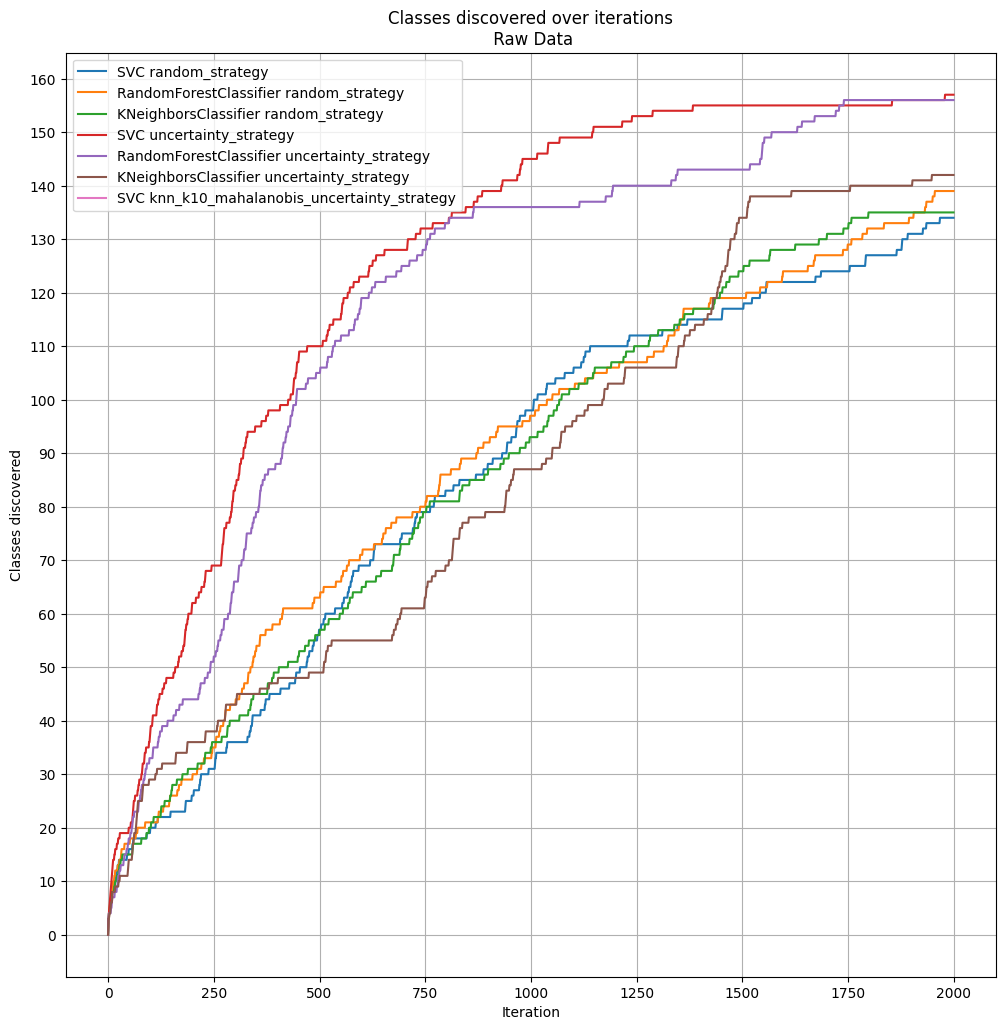
\includegraphics[width=0.9\textwidth]{resources/images/rev2_classes_discovered_raw_data.png}
\caption{Raw Data Classes Discovered}
\label{fig:classes_discovered_begin}
\end{figure}

\begin{figure}[htbp]
\centering
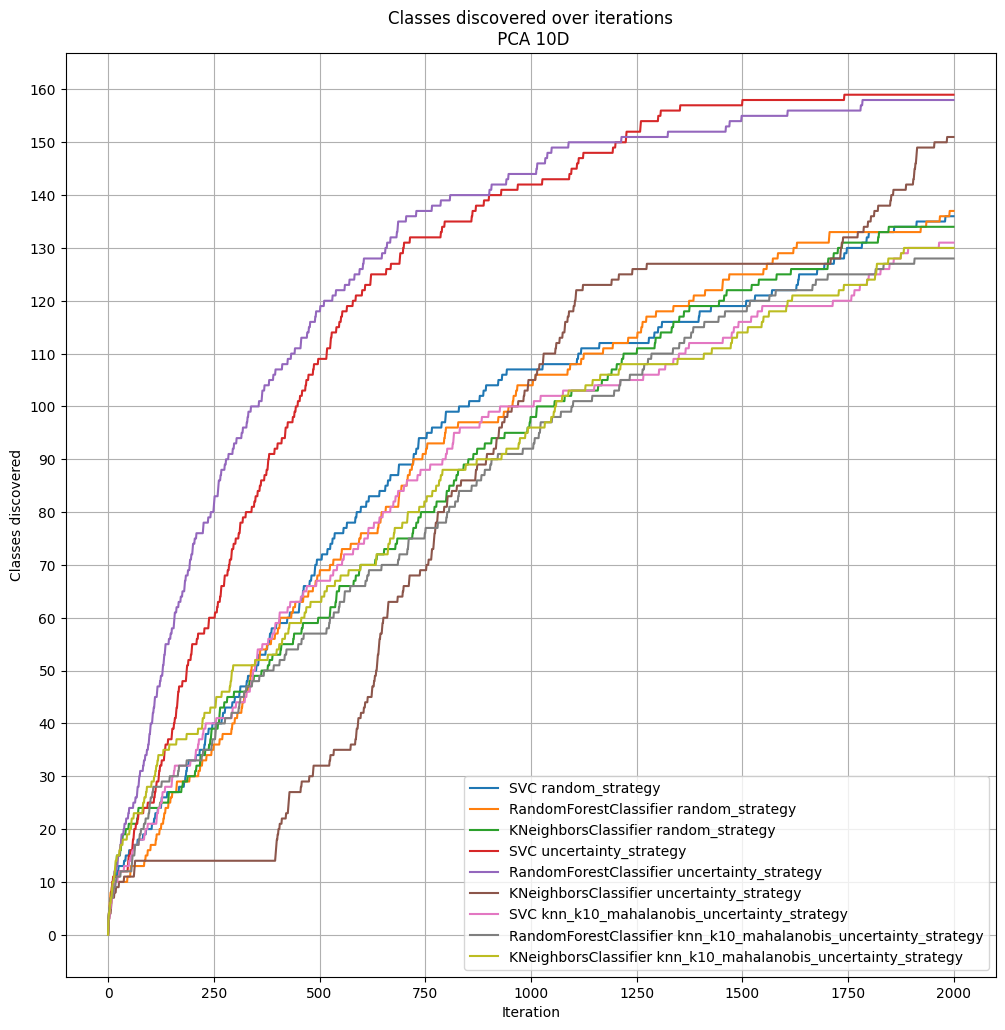
\includegraphics[width=0.9\textwidth]{resources/images/rev2_classes_discovered_10d.png}
\caption{10D PCA Classes Discovered }
\end{figure}

\begin{figure}[htbp]
\centering
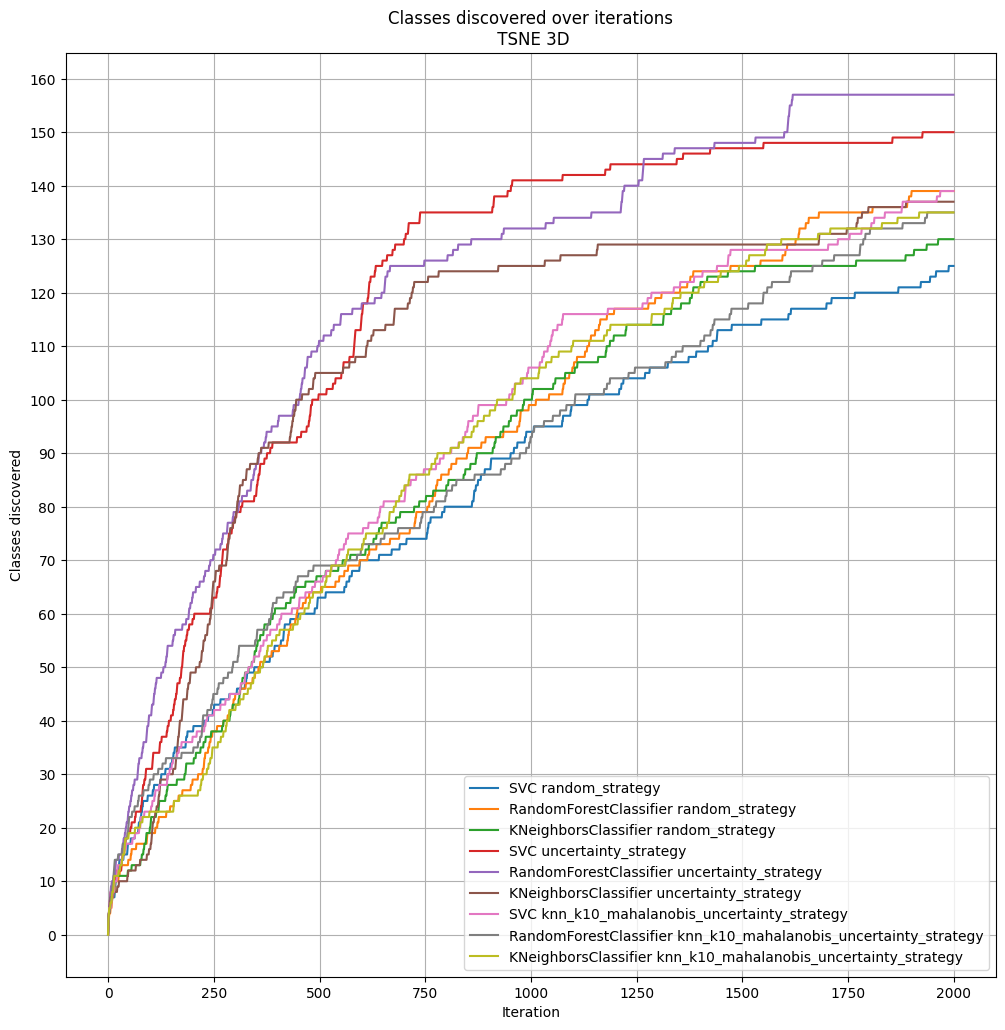
\includegraphics[width=0.9\textwidth]{resources/images/rev2_classes_discovered_tsne3d.png}
\caption{3D t-SNE Classes Discovered}
\end{figure}

\begin{figure}[htbp]
\centering
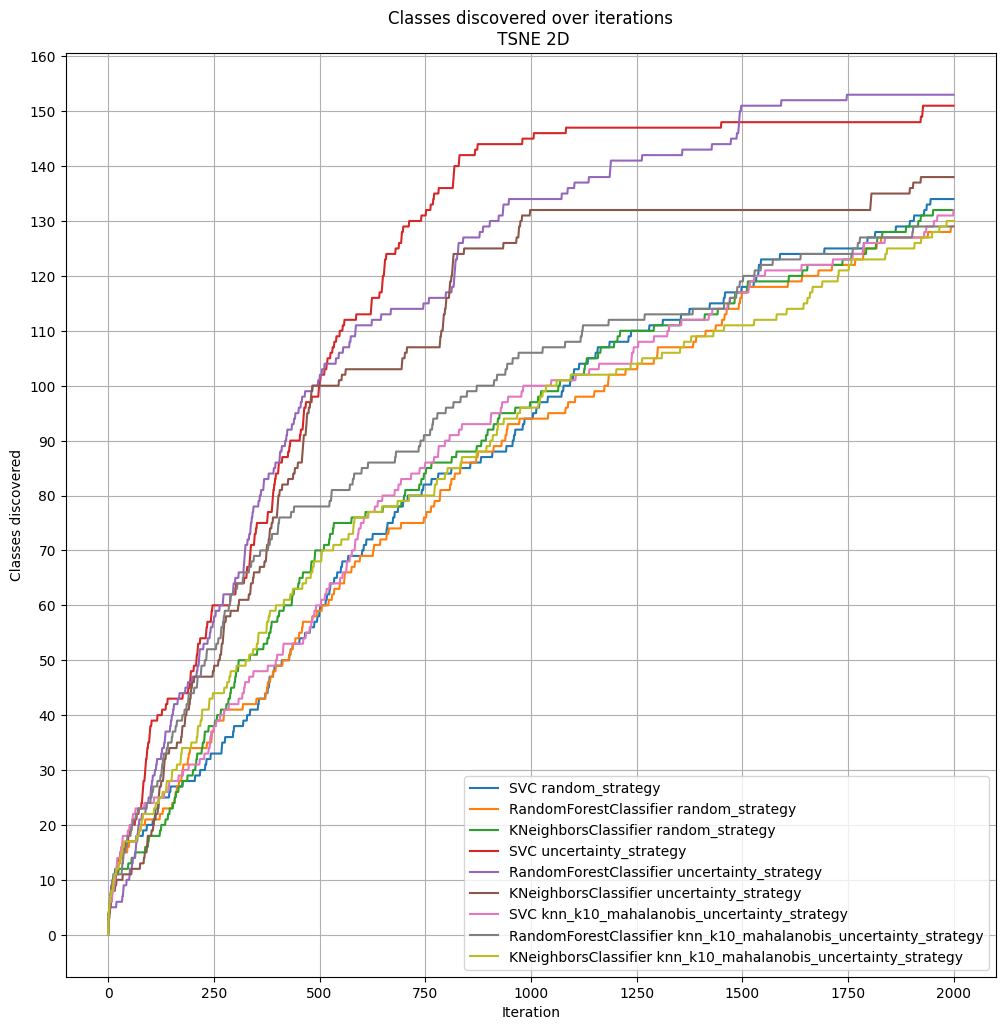
\includegraphics[width=0.9\textwidth]{resources/images/rev2_classes_discovered_tsne2d.png}
\caption{2D t-SNE Classes Discovered}
\end{figure}

\begin{figure}[htbp]
    \centering
    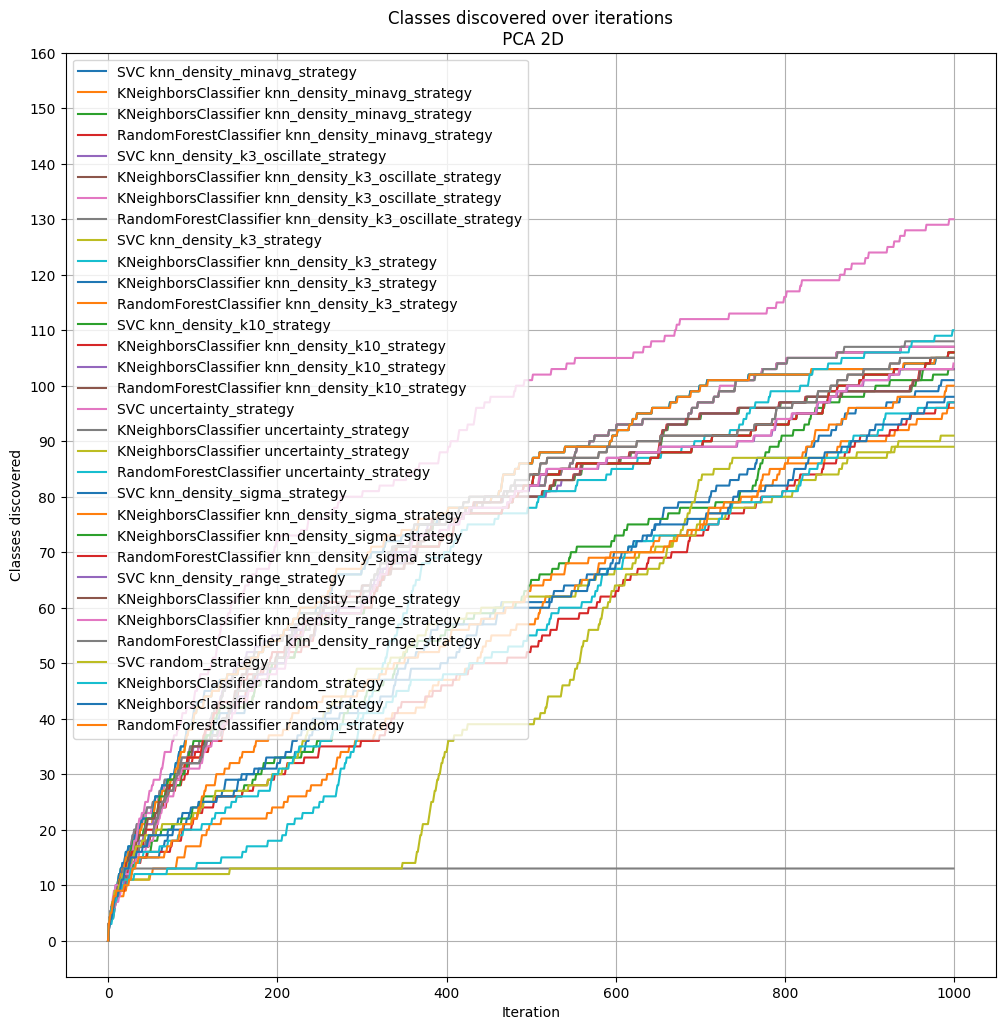
\includegraphics[width=0.9\textwidth]{resources/images/classes_discovered_pca_2d.png}
    \caption{2D PCA Classes Discovered on original algorithms}
\end{figure}

\begin{figure}[htbp]
    \centering
    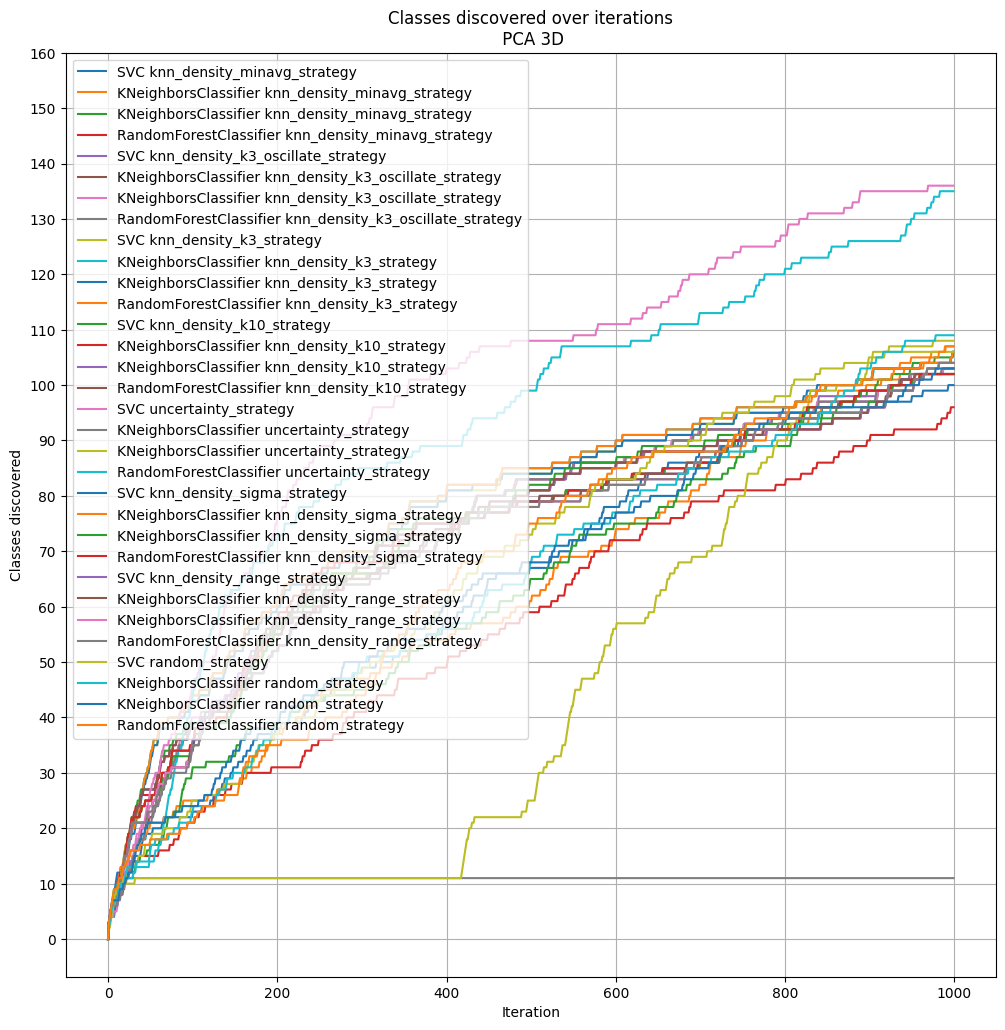
\includegraphics[width=0.9\textwidth]{resources/images/classes_discovered_pca_3d.png}
    \caption{3D PCA Classes Discovered on original algorithms}
\end{figure}

\begin{figure}[htbp]
    \centering
    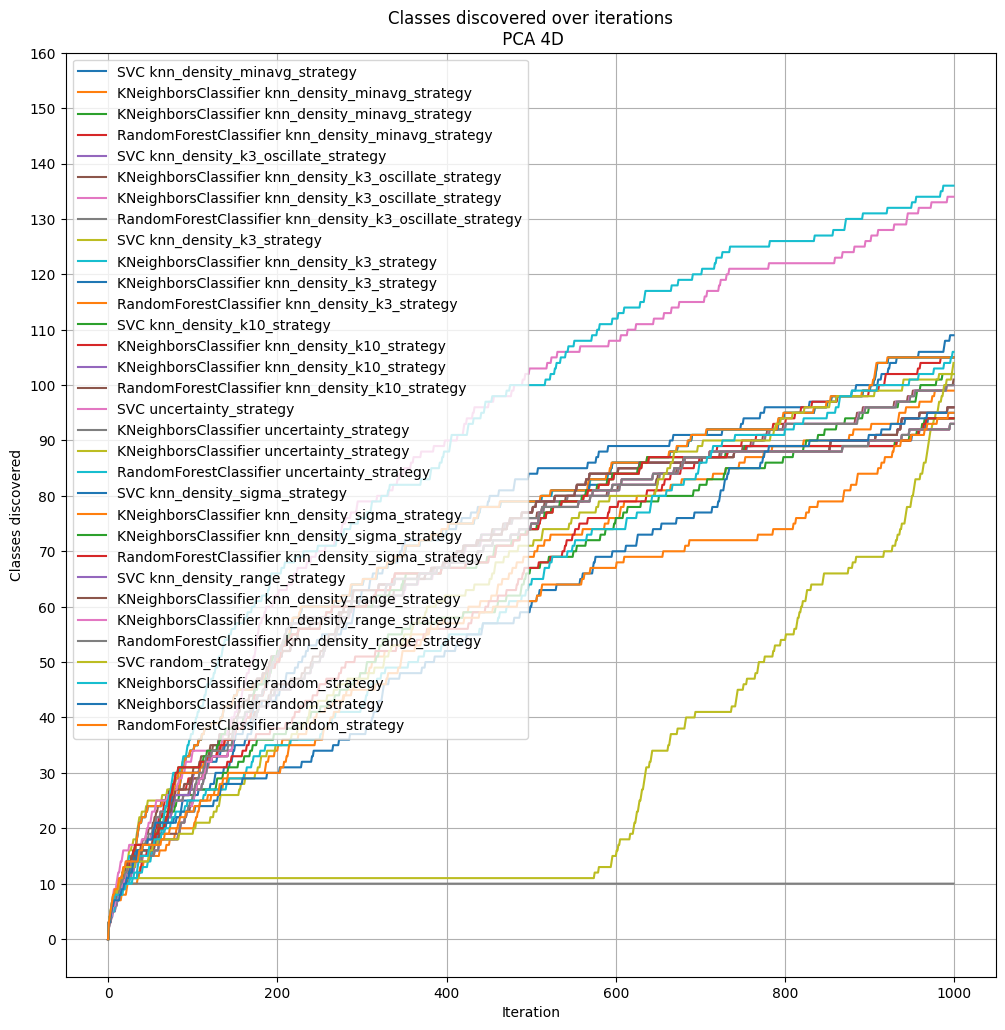
\includegraphics[width=0.9\textwidth]{resources/images/classes_discovered_pca_4d.png}
    \caption{4D PCA Classes Discovered on original algorithms}
\end{figure}

\begin{figure}[htbp]
    \centering
    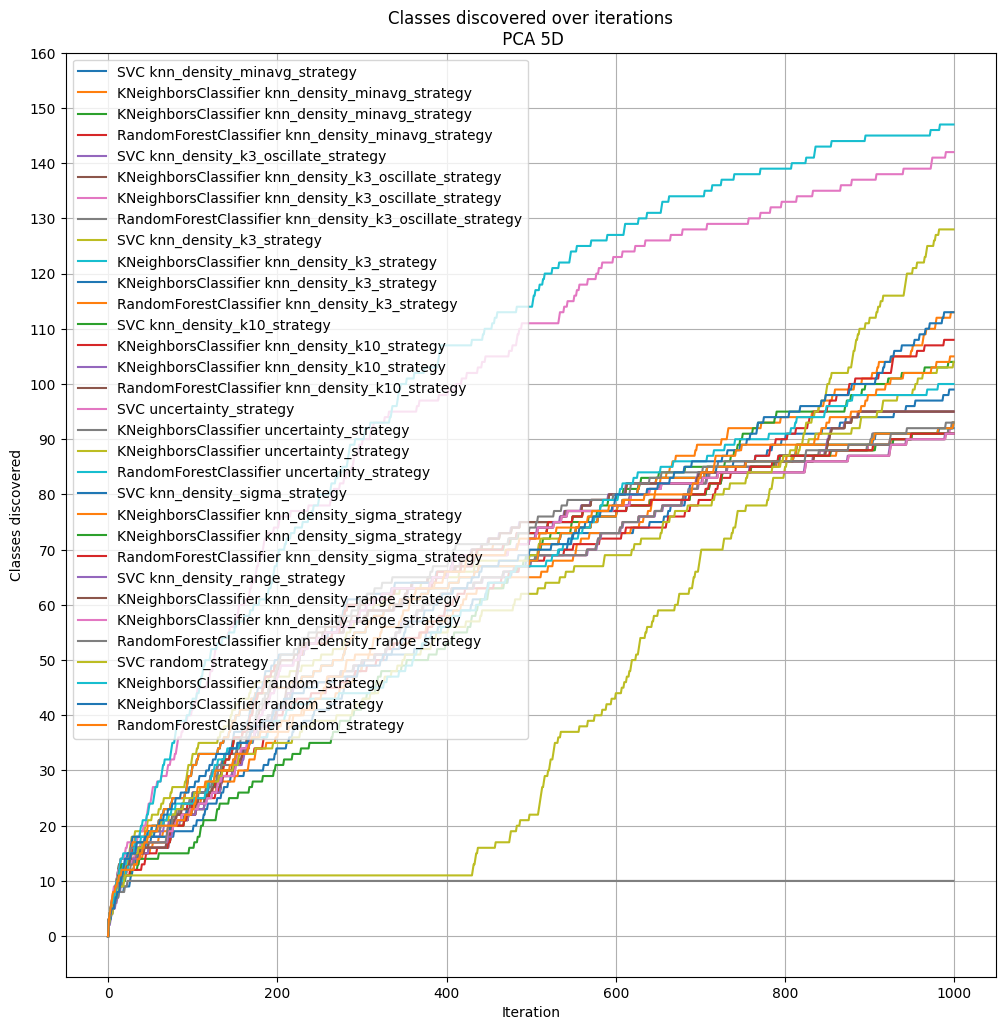
\includegraphics[width=0.9\textwidth]{resources/images/classes_discovered_pca_5d.png}
    \caption{5D PCA Classes Discovered on original algorithms}
\end{figure}

\begin{figure}[htbp]
    \centering
    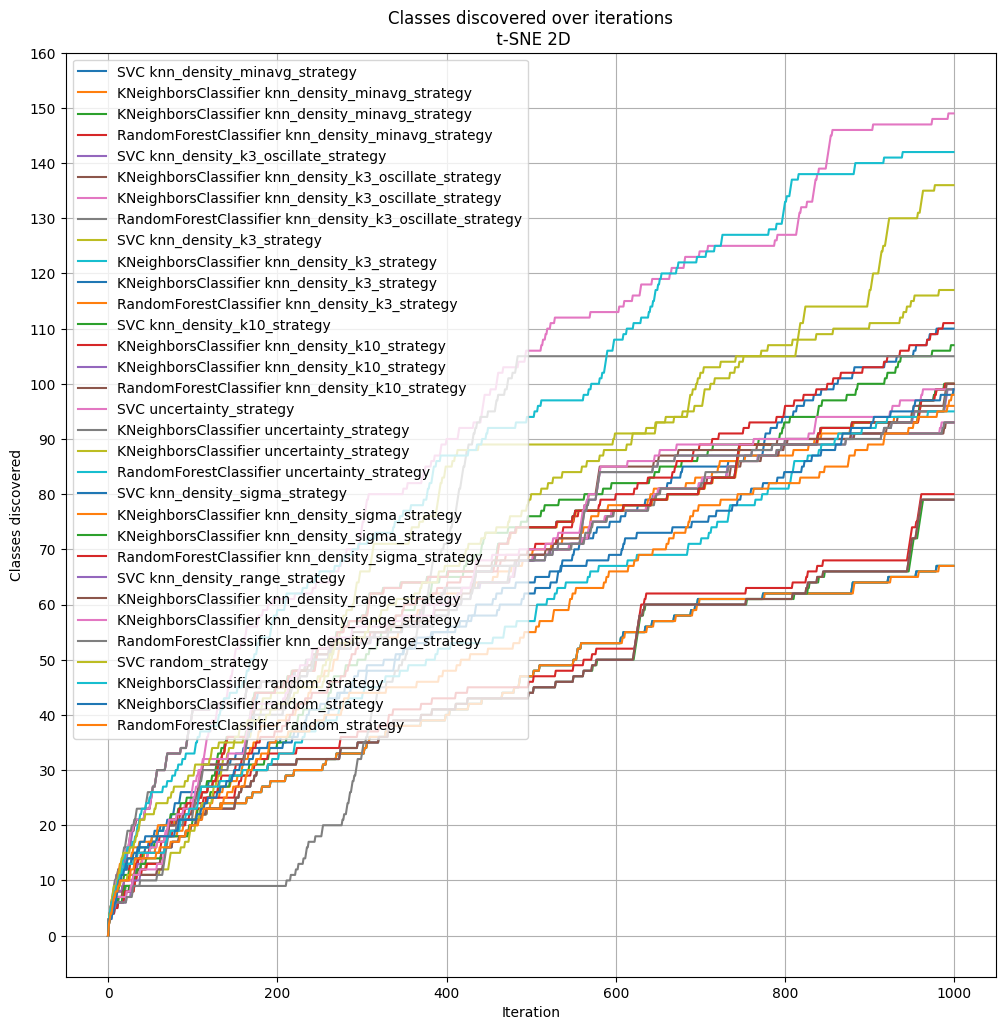
\includegraphics[width=0.9\textwidth]{resources/images/classes_discovered_tsne_2d.png}
    \caption{2D t-SNE Classes Discovered on original algorithms}
\end{figure}

\begin{figure}[htbp]
    \centering
    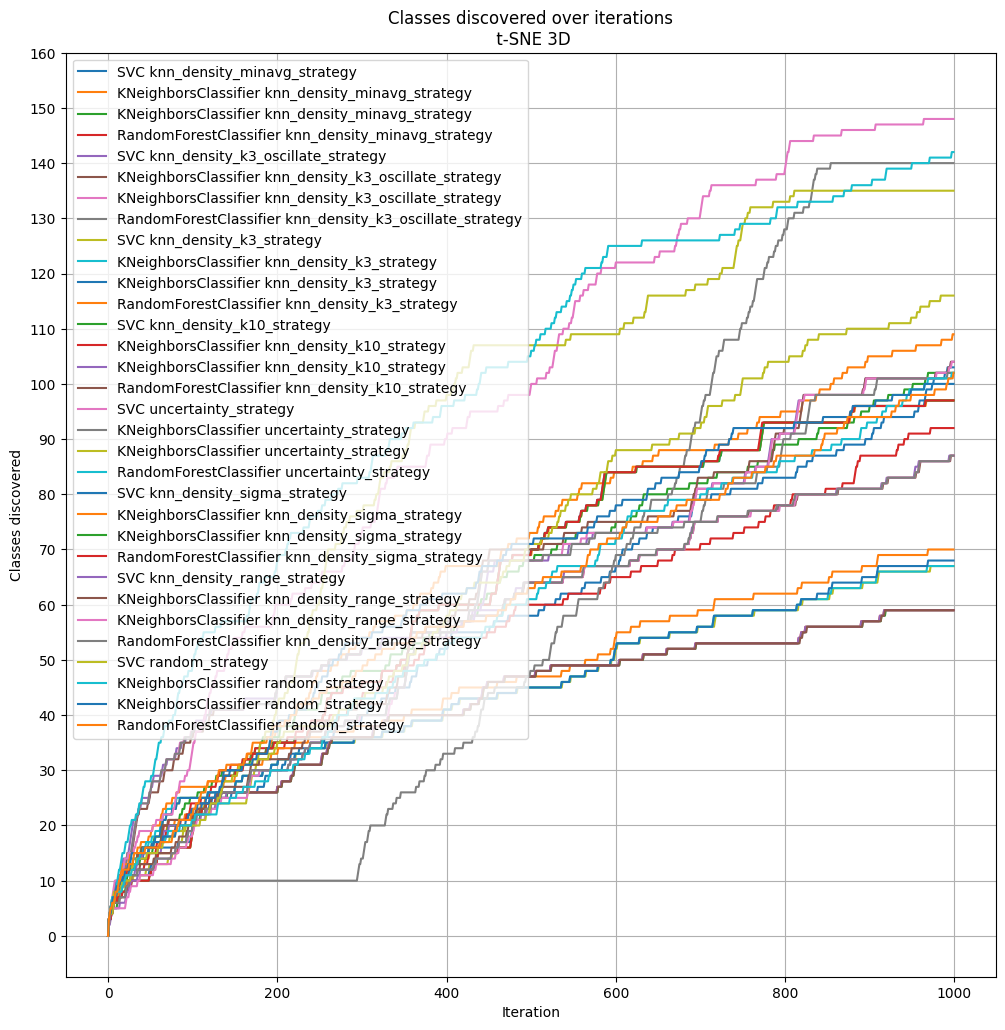
\includegraphics[width=0.9\textwidth]{resources/images/classes_discovered_tsne_3d.png}
    \caption{3D t-SNE Classes Discovered on original algorithms}
    \label{fig:classes_discovered_end}
\end{figure}


\newpage
%\appendixname{Python Requirements}

\twocolumn
Python Requirements\par
asttokens==2.4.1\par
colorama==0.4.6\par
comm==0.2.2\par
contourpy==1.2.1\par
cycler==0.12.1\par
debugpy==1.8.1\par
decorator==5.1.1\par
executing==2.0.1\par
fonttools==4.51.0\par
graphviz==0.20.3\par
ipykernel==6.29.4\par
ipython==8.23.0\par
jedi==0.19.1\par
joblib==1.4.0\par
jupyter$\_$client==8.6.1\par
jupyter$\_$core==5.7.2\par
kiwisolver==1.4.5\par
matplotlib==3.8.4\par
matplotlib-inline==0.1.7\par
nest-asyncio==1.6.0\par
numpy==1.26.4\par
packaging==24.0\par
pandas==2.2.2\par
parso==0.8.4\par
pillow==10.3.0\par
platformdirs==4.2.0\par
prompt-toolkit==3.0.43\par
psutil==5.9.8\par
pure-eval==0.2.2\par
Pygments==2.17.2\par
pyparsing==3.1.2\par
python-dateutil==2.9.0.post0\par
pytz==2024.1\par
pywin32==306\par
pyzmq==26.0.0\par
scikit-learn==1.4.2\par
scipy==1.13.0\par
six==1.16.0\par
stack-data==0.6.3\par
threadpoolctl==3.4.0\par
tornado==6.4\par
traitlets==5.14.2\par
tzdata==2024.1\par
wcwidth==0.2.13\par
